\iffalse \bibliography{include/backmatter/magnus,include/backmatter/philip} \fi

\chapter{Background \& Related Work} \label{sect:background} 
In this section we introduce (i) technological concepts related to this study, (ii) the process of identifying related work and (iii) discuss current research on scope of this study. This section aims to present background information on this study and related work for readers to familiarise with. 

\todo{why is this section important?}
%This section aims to explore literature on using lightweight containers for deployment. 
% aims to show how this research fits into a larger research context 

\section{Background}
%---------------------------------------------------%
\subsection{Cyber Physical Systems}
%compact middle-ware OpenDaVINCI written in standard C++, can be used on a variety of POSIX OS. we use ODV to have a lean, portable and high-performance hardware and OS abstraction layer for typical programming idioms like concurrency, data storage and communication

Comparing a real-time system with an ordinary application, the difference is seen in how the execution of code is made. For an ordinary application an algorithm is executed once to provide a result output from an input without any specific time constraints. However, a real-time system is recognised by its time constrain characteristic as the system is configured to execute an algorithm within a specified time-slice, i.e. \texttt{10milliseconds}.\\

Systems used for autonomous self-driving vehicles utilises a number of different algorithms to enable the self-driving functionality. The responsibilities for these algorithms is presented in figure \ref{containers}, where different responsibilities are broken down. One algorithm is responsible for processing the camera feed, another algorithm is responsible for detecting lanes within the captured images from the camera, and another is responsible for make a decision to steer, break, or accelerate the vehicle depending on the content of the feed. All these algorithms are embedded in a middle-ware application which sets the time constraints of the algorithms and handle the interface between the different nodes. This research looks to utilise an open source middle-ware named OpenDaVINCI. OpenDaVINCI is an application specifically developed for autonomous self-driving vehicles which is implemented in several research projects \cite{OpenDaVINCI}.
%---------------------------------------------------%
\subsection{Software Deployment}
%Software deployment for CPS is difficult as there are many aspects to put into consideration. Typically,  CPS are resource constrained, meaning that you cannot scale up hardware exponentially as you typically do not have the physical space for it. Secondly, real-time requirements are needed, so any SD tools needs to be lightweight. Finally, there are safety concerns since CPS typically interact with their surroundings. 

Software deployment is a crucial part of the software development, it refers to the activities which makes the software system available for use \cite{carzaniga1998characterization}. The process contains a number of activities which all play into the life cycle of a software system with the goal to implement into the runtime environment where the system is set to operate live. These activities are namely: \\

\textbf{Release} – is the activity of packaging the software for delivering it to the end user. This includes processes such as including the software's requirements and dependencies to external components, such as libraries and applications. It also includes the process of advertising – the process of informing interested parties about the software being released.\\
\textbf{Install} – refers to the activities of assembling all required resources for the runtime environment. It consists of two specific process, namely \textit{transfer} and \textit{configuration}. Where the former is the process of transferring the software from the developer to the runtime environment and the later is the process of making the software ready for activation.\\
\textbf{Activate} – is the process of executing the software and all dependent applications in the runtime environment.\\
\textbf{Deactivate} – is the opposite of the \textit{activate} activity.\\
\textbf{Update} – is the activity of updating the version of the running software which consists of similar activities of the \textit{install} activity.\\
\textbf{Adapt} – refers to the process of ensuring that the updated version is running correctly in the runtime environment.\\
\textbf{Deinstall} – is the activity of decommissioning the running software and includes sub-activities such as removing the external libraries and components.\\
\textbf{Derelease} – is the final activity which includes the process of advertising the withdrawal of the software system.\\

All these activities differ in how they are executed depending on the software engineering paradigm utilised for the software project. In traditional software engineering practices, e.g. the waterfall model, seeks to execute the software deployment process at the end of the software's development cycle. Whereas more novel software engineering practices aim to execute the software deployment process continuously throughout the software's development cycle. In state-of-art software engineering practices such as continuous integration and continuous deployment, requires software to be deployed daily \cite{meyer2014continuous}. Such requirements can easily make the process of software deployment exhausting and complex, where software tools such as Docker would simplify these processes greatly. Docker simplifies processes found within each of the software deployment activities, as it provides the runtime environment before the software deployment process has begun. The development environment is a clone of the production environment thus transferring the deployment processes from the live production server to a confined a secure location where the deployment process does not affect the usability of the current running software.\\


\begin{figure}[ht]
\centering
     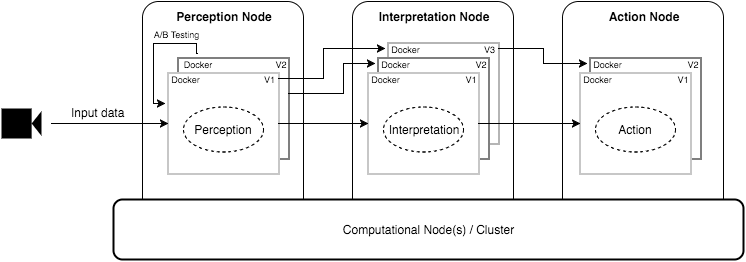
\includegraphics[width=1.0\textwidth]{./figure/containers.png}
      \caption{Run-time environment using Docker.}
       \label{containers}
\end{figure}

Figure \ref{containers} displays a deployment strategy design utilising Docker in the context of self-driving vehicles. The responsibilities are broken down into three computational nodes in which Docker containers are running instances of the code base independently. Each Docker container can run different versions of the separate nodes, where the interpretation node has three versions running separately. Version one (denoted V1) in each node represents the latest working configuration while other versions are run to test code which is still under development. Aforementioned, this allows for safe and simple roll-backs in the event of buggy code or degraded performance. Furthermore, multiple versioning of the same Docker container allows for split testing between different containers to take place. With an always functioning configuration, the development team can demonstrate the current status to stakeholders at any point in the development cycle. The ability to demonstrate the product at any point in the development phase adds to the business value as possible investors or stakeholders can see a functioning product even though it is currently under development. With current approaches this is possible, however it is not as straightforward and easily implemented as in cases which utilizes Docker for its deployment strategy.
%---------------------------------------------------%
\subsection{Container-Based Virtualization}
%process isolation and application portability
%virtualization can be done with fully-fledged Virtual Machines or lightweight containers. VMs  incure higher ovhead but better protection and so are not suitable for autonomous vehicles.  Therefore we adopt containers and strive to minimize latency by real-time Linux kernel
%containers very efficiently share and utilize CPU and memory resources, 

Docker is an open source light-weight container environment which was initially launched in 2013 and has gained ground rapidly with its simplicity. The environment offered by Docker simplifies the process of software deployment by packaging all dependencies into a light-weight virtualization container which ensures that all instances of the software is utilising the same dependent libraries. The functionality provided by Docker is comparable with virtual machines as both are virtualised environments where software applications can be executed with all dependent libraries and applications are installed. However, Docker, in contrast to virtual machines, is a light-weight alternative as it communicates directly to the host machine's kernel. A virtual machine has the additional level of a virtual operating system which adds complexity which does not directly speak with the host machine's kernel. With the benefit of packaging the dependent libraries and applications into the container, software developers can avoid uncertain deployments where library versions may differ between the developers' development environments and the live production environment. Docker presents further benefits such as safe roll-back between different software versions which provides projects' the ability to always be able to fall back on application versions which are known to function correctly. By providing these benefits project managers can feel secure in that there always exists a working runtime environment in the scenario of a new failing deployment.\\

The container in which Docker packages all dependent libraries and applications are referred to as a Docker image. This image contains everything which is required for an application to be executed. In the case of self-driving vehicles such dependencies may be image processing libraries such as OpenCV and the middle ware which enables the real-time application. When executing an application within Docker, a container is executed with based on the Docker image which consists of the installed libraries. This software design allows for split testing of software as the same application can be executed multiple times without clashing with the other contained application. Thus being optimal for testing different versions of the same application simultaneously while knowing there is no interference between the executed applications.
%---------------------------------------------------%
\subsection{Task Scheduling} 
%kernel and cpu scheduler
An operating system handles the communication between the software and the hardware, more specifically the operating system kernel acts as the interface between hardware and software. As an operating system is running a vast amount of processes simultaneously there is a need to prioritise and select which processes to run at what time. Each process utilises the CPU to make the computations required for the process to operate. The CPU is a powerful piece of hardware which can handle the same number of processes as it has cores and threads, i.e. an general Intel Core i7 processor has 4 cores and two threads per core amounting to 8 total processes simultaneously. However an operating system may run more processes than the CPU can process simultaneously. To manage this flood of processes a software component referred to as the \textit{CPU scheduler} which is configured by the kernel and is implemented to ensure that there is a queuing system set up for all processes running on the system. The \textit{CPU scheduler} acts as a traffic police in a busy intersection, handling a queue of all the processes running on the system by prioritising some processes ahead of other processes. The \textit{CPU scheduler} may act and prioritise differently depending on what rules have been set for it to follow.\\

The Linux OS CPU scheduler implements a FIFO (first-in-first-out) approach with two process scheduler algorithms, namely a time-sharing algorithm and a real-time algorithm. Where the former is a \textit{fair} scheduler algorithm trying to distribute the system's CPU resources equally over all processes in the queue ensuring that no process is completely starved. The later is an algorithm which prioritises the processes based on their set importance, where a higher prioritised process is provided more resources in comparison with a lower process. However, the generic Linux kernel version does not allow for any resource cut-off for processes utilising the CPU. A higher prioritised process will therefore not be able to utilise 100\% of the CPU's resources if there are other processes already using the CPU. This is not remarkable for a general purpose operating system running non-time sensitive applications. For a RT system it is crucial to ensure that the highest level process can interrupt any running processes at any point in time. An RT\_preempt kernel may be implemented to cope with such a design. This kernel design allows the scheduler to preempt any running process of lower priority than the requested process. Furthermore, the RT\_preempt kernel locks any resource utilised by a RT prioritised process.
%---------------------------------------------------%
\subsection{Real Time System and Scheduling Precision}
%latency mitigated by modifying operating sytem to provide more determinism 
%linux foundation announced fully support rt linux 
To understand the performance impact of utilizing Docker containers for the deployment strategy, the experiments of this research will analyse the scheduling precision of the automotive real-time application. The application executes computations within elements referred to as time-slices. The time-slice is a specification of time allocated for the algorithm to execute and deliver a result. A real-time application running at \texttt{100hertz} executes 100 time-slices per second, which results in one time-slice being \texttt{10milliseconds} or \texttt{0.01second}. The \texttt{10milliseconds} time-slice is the time deadline set for the specific application, which is the maximum time allowed for the assigned algorithm to finish its computations. In scenarios where the algorithm utilizes less than the assigned time-slice the application will sleep for the remaining time until it fires a new execution. Assuring that the application sleeps for the specified time is a responsibility assigned to the operating system scheduler. Where the scheduler initiates processes which are sleeping and wishes to fire a new time-slice. Other than the assigned algorithm, the real-time application consists of code which is responsible for controlling the sleep of the time-slices. Therefore a part of the time-slice has to be consumed to execute the required code. The time consumed by the code which controls the sleep of the application is referred to as the middle-ware overhead which is part of what is used for measuring the scheduling precision of the execution environment.\\

Scheduling precision refers to how accurately the application executes the specified algorithm from the point of firing the time-slice until the algorithm begins its computation. Further accuracy is measured between the point of where the algorithm finishes its computations until the real-time application sleeps. Lastly, measurements are done to see whether the \texttt{sleep} function of the system actually sleeps for the remainder of the time-slice or if it overstays the specified time deadline.\\

The limitations of each execution environment can be identified by understanding how much time each part of the required code occupies the time-slice. The less time required for executing the code outside of the assigned algorithm the more deterministic a system is said to be. In a scenario where the assigned algorithm requires 80\% of the time-slice to execute the code, it is assumed that the application will sleep for the remaining 20\%. However, as there exists additional operations surrounding the algorithm the application might sleep 18\% whereas 2\% is required for the surrounding code to execute. If the application still sleeps 20\%, executes the algorithm for 80\%, and uses 2\% for the required code it will overstay its time-slice by 2\% thus rendering the application less deterministic. It is the time available for the algorithm the experiments will seek to identify to inform software engineers of how much of the time-slice can be used for effective computations, i.e. time available for generating a result.





%---------------------------------------------------%
%---------------------------------------------------%
\section{Gathering Related Work}
The snowballing search approach for systematic literature studies is used to find relevant literature on the topic of this paper. The snowballing approach is complementary to a traditional database search. Specifically, the reference list and citations of a paper are studied in order to identify additional papers. The snowballing search approach is used to ensure good coverage of current literature.\\

The guidelines for conducting a snowballing search approach, presented by Wohlin \cite{Wohlin} are followed. The steps to conduct a snowballing procedure involve selecting a start set of papers and apply forward and backward snowballing on each paper respectively. The process iterates until no new papers are found. To identify a start set of papers, keywords are extracted from the research questions, taking synonyms into account. Formulating a search-string from keywords that are broad and cover multiple areas of research may result in collecting large amounts of literature that span different subject domains. For that reason, broad keywords should be broken down into more specific and detailed keywords specific to the study. The search string is then applied to a database that preferably searches multiple publishers in order to avoid publisher bias. The papers are then screened according to inclusion/exclusion criteria. An exclusion criteria could state that all online material be excluded. \\

Backward and forward snowballing is then conducted on the start set. Backward snowballing is the process of studying the reference list to identify new papers. Looking at the place of reference and reading the title and abstract of the paper is a good starting point for inclusion, however, final inclusion states that the entire paper must be read. Subsequently, forward snowballing is the identifying papers that cite the paper under inspection. The same process of reading the title, abstract and place of reference is applied in order to include new literature. 

%-- Why Snowballing ?
%snowballing to ensure good coverage of literature
%snowballing over just a typical database search
%since we're writing about new tech, new papers must certainly reference at least one paper among previously releant studies

%-- Outline the steps in snowballing
%let’s outline them here, so the steps are clear. (what are iterations)
%Then, you describe the steps and their outcomes. 
%A figure showing the process could be used if you judge it fits

%-------------------------------
\subsection{Snowballing Search Results}
This section introduces the results from performing the snowballing search procedure described in the previous section. First the start-set is formulated and introduced, where two sets of iterations are performed. 

\subsubsection*{Start Set}
A database search on Scopus \cite{scopus} is performed to identify the start set: the search string is found in \ref{search-string}.  The actual search was conducted May 10, 2016. The Scopus database returns literature from multiple publishers. The search resulted in finding 215 papers. The screening process was then applied to the 215 papers. Papers were added to the start set upon meeting the inclusion/exclusion criteria. Papers were included if found to be about input/output benchmarking, CPU benchmarking or software deployment, within the subject area of virtual containers (preferably Docker) and/or within the context of cyber physical systems. Papers were excluded if not being peer-reviewed. In total, 10 candidates for inclusion were identified. The 10 papers are identified in table~\ref{lr-startset}, denoted P1, P2 and so on.

\begin{table}[]
\centering
\begin{tabular}{p{15cm}}
TITLE-ABS-KEY(Performance OR Comparison OR Latency OR Evaluation OR Container-Based OR Linux Containers OR Lightweight Virtualization OR Container Cloud OR Docker) AND ( LIMIT-TO(SUBJAREA,"COMP" ) )
\end{tabular}
\caption{Search String}
\label{search-string}
\end{table}

%-----------------------%
\begin{table}[]
\begin{tabular}{lp{13cm}}
{[}P1{]}  & C. N. Mao, M. H. Huang, S. Padhy, S. T. Wang, W. C. Chung, Y. C. Chung, and C. H. Hsu, “Minimizing latency of real-time container cloud for software radio access networks,” in 2015 IEEE 7th International Conference on Cloud Computing Technology and Science (CloudCom), Nov 2015, pp. 611–616.                                  \\
{[}P2{]}  & A. Krylovskiy, “Internet of things gateways meet linux containers: Performance evaluation and discussion,” in Internet of Things (WF-IoT), 2015 IEEE 2nd World Forum on, Dec 2015, pp. 222–227.                                                                                                                                      \\
{[}P3{]}  & M. Raho, A. Spyridakis, M. Paolino, and D. Raho, “Kvm, xen and docker: A performance analysis for arm based nfv and cloud computing,” in Information,Electronic and Electrical Engineering (AIEEE), 2015 IEEE 3rd Workshop onAdvances in, Nov 2015, pp. 1–8.                                                                         \\
{[}P4{]}  & R. Morabito, J. Kj\"allman, and M. Komu, “Hypervisors vs. lightweight virtualization: A performance comparison,” in Proceedings of the 2015 IEEE Interational Conference on Cloud Engineering, ser. IC2E ’15. Washington, DC, USA: IEEE Computer Society, 2015, pp. 386–393.                                                      \\
{[}P5{]}  & M. G. Xavier, I. C. D. Oliveira, F. D. Rossi, R. D. D. Passos, K. J. Matteussi, and C. A. F. D. Rose, “A performance isolation analysis of disk-intensive workoads on container-based clouds,” in 2015 23rd Euromicro International Conference on Parallel, Distributed, and Network-Based Processing, March 2015, pp. 253–260. \\
{[}P6{]}  & W. Felter, A. Ferreira, R. Rajamony, and J. Rubio, “An updated performance comparison of virtual machines and linux containers,” in Performance Analysis of Systems and Software (ISPASS), 2015 IEEE International Symposium on, March 2015, pp. 171–172.                                                                            \\
{[}P7{]}  & C. Ruiz, E. Jeanvoine, and L. Nussbaum, “Performance evaluation of containers for hpc,” in Euro-Par 2015: Parallel Processing Workshops: Euro-Par 2015 International Workshops, Vienna, Austria, August 24-25, 2015, Revised Selected Papers. Cham: Springer International Publishing, 2015, pp. 813–824. \\
{[}P8{]}  & R. Wu, Y. Chen, E. Blasch, B. Liu, G. Chen, and D. Shen, “A container-based elastic cloud architecture for real-time full-motion video (fmv) target tracking,” in 2014 IEEE Applied Imagery Pattern Recognition Workshop (AIPR), Oct 2014, pp. 1–8.                                                                                  \\
{[}P9{]} & Z. Estrada, F. Deng, Z. Stephens, C. Pham, Z. Kalbarczyk, and R. Iyer, “Performance comparison and tuning of virtual machines for sequence alignment software,” Scalable Computing, vol. 16, no. 1, pp. 71–84, 2015.
\end{tabular}
\centering
\caption{Start Set}
\label{lr-startset}
\end{table}
%-----------------------%
%------Iteration 1------ 
\subsubsection*{Iteration 1: Backward Snowballing}
\textbf{P1} includes 26 references where one reference is already included in the start set (paper P6). Based on the inclusion criteria, one paper was included. The paper identified and thus included in the start set is: \\

%-------------------------------
\begin{labeling}{[{[}C10{]}]}
\item [{[}\textbf{C1}{]}]  M. G. Xavier, M. V. Neves, F. D. Rossi, T. C. Ferreto, T. Lange and C. A. F. De Rose, “Performance Evaluation of Container-Based Virtualization for High Performance Computing Environments,“ 2013 21st Euromicro International Conference on Parallel, Distributed, and Network-Based Processing, Belfast, 2013, pp. 233-240.
\item
\end{labeling}
%-------------------------------

Table~\ref{back-snow} shows the result of backward snowballing on the remaining eight papers. The results are presented in a table to avoid redundant text as the process and results of backward snowballing for each paper are very similar. In all papers, except P1, no new papers matched the inclusion criteria after reading the title and abstract. Furthermore, most of the papers in the start set reference to each other, as seen in column three of table~\ref{back-snow}. All papers in the start set contain reference to C1, except papers P2 and P8. Similarly, all papers in the start set reference to P6 except papers P5, P6 and P8. This shows that there is a strong connection between all papers in the start set. 

%-------------------------------
\begin{table}[]
\begin{tabular}{|>{\centering\bfseries}m{1in} |>{\centering}m{1in}| >{\centering}m{1in} |>{\centering\arraybackslash}m{1in}|}
\hline
\textbf{Start Set Paper} & \textbf{No. References} & \textbf{Reference to Start Set} & \textbf{New Papers Identified} \\ \hline
\textbf{P1}              & 26                      & P6                                          & C1                  \\ \hline
\textbf{P2}              & 21                      & P6, P4                                      & 0                   \\ \hline
\textbf{P3}              & 47                      & P6, C1                                      & 0                   \\ \hline
\textbf{P4}              & 42                      & P6, P2, C1                                  & 0                   \\ \hline
\textbf{P5}              & 46                      & C1                                          & 0                   \\ \hline
\textbf{P6}              & 50                      & C1                                          & 0                   \\ \hline
\textbf{P7}              & 19                      & P6, C1                                      & 0                   \\ \hline
\textbf{P8}              & 18                      & 0                                           & 0                   \\ \hline
\textbf{P9}              & 31                      & P6, C1                                      & 0                   \\ \hline
\end{tabular}
\centering
\caption{Results from Backward Snowballing in Iteration 1}
\label{back-snow}
\end{table}
%-------------------------------

\subsubsection*{Iteration 1: Forward Snowballing}
The next step is to examine the citation to all papers that are in the start set. All papers were searched for citations using Google Scholar. The Scopus database was chosen not to be used for the forward snowballing procedure since it was shown that Google Scholar was more accurate in finding cited papers. The exclusion criteria for this snowballing search procedure excludes all non peer reviewed papers. However, during the forward snowballing search, a very relevant paper was found in regards to this study. It was then decided to include the paper as part of the related work. The specific paper included is: \\


\begin{labeling}{[{[}C10{]}]}
\item [{[}\textbf{C2}{]}]  Welch, James Matthew. Performance Optimization of Linux Networking for Latency-Sensitive Virtual Systems. Diss. ARIZONA STATE UNIVERSITY, 2015.

\item
\end{labeling}

\begin{table}[]
\begin{tabular}{|>{\centering\bfseries}m{1in} |>{\centering}m{1in}|>{\centering\arraybackslash}m{1in}|}
\hline
\textbf{Start Set Paper} & \textbf{No. Citations}  & \textbf{New Papers Identified} \\ \hline
\textbf{P1}              & 0                       & 0                             \\ \hline
\textbf{P2}              & 0                       & 0                             \\ \hline
\textbf{P3}              & 0                       & 0                             \\ \hline
\textbf{P4}              & 8                       & C2				               \\ \hline
\textbf{P5}              & 2                       & 0                             \\ \hline
\textbf{P6}              & 81                      & 0                             \\ \hline
\textbf{P7}              & 4                       & 0                             \\ \hline
\textbf{P8}              & 1                       & 0                             \\ \hline
\textbf{P9}              & 1                     & 0                             	\\ \hline
\end{tabular}
\centering
\caption{Results from Forward Snowballing in Iteration 1}
\label{forward-snow}
\end{table}

\subsubsection*{Iteration 2: Backward Snowballing}
Two additional papers to the start set were found in iteration one of the snowballing procedure. Thus, backward and forward snowballing is applied to C1 and C2.\\ 

\textbf{C1} has 32 references. Of the 32 references, 16 references are excluded based on being references to online material. A large number of the resulting references have already been analysed in the previous iteration. No new papers were identified for inclusion.\\ 

\textbf{C2} has 69 references with reference to C1, P4, P6. No additional papers were found when studying the reference list of the paper.

\subsubsection*{Iteration 2: Forward Snowballing}
\textbf{C1} has been cited by 104 papers. When reviewing the list of cited papers, many of them have already been reviewed during the snowballing procedure.  Analysing the list of papers resulted in no additional candidates for inclusion.\\ 
 
\textbf{C2} has no citations. This is expected since C2 is not a published paper. 


\subsection{Outcome}
The snowballing search procedure resulted in finding nine papers during the database search. Two additional papers were identified during forward and backward snowballing. The snowballing procedure enabled good coverage of literature for related work and helped identify the current status of research in the field of container virtualization. 
%a qualitative outcome of the snowballing procedure. What did it actually give us, and do for the paper? 
%However, since there was only one new paper included in the start-set during the backward snowballing, this sheds light on the fact that this study is within a narrow scope, and further motivates the need for carrying out this study. 

%What did we get out of doing the snowballing

\section{Related Work} 
\todo{can we have the same heading here again?}




